\section{Circuits} \begin{figure} 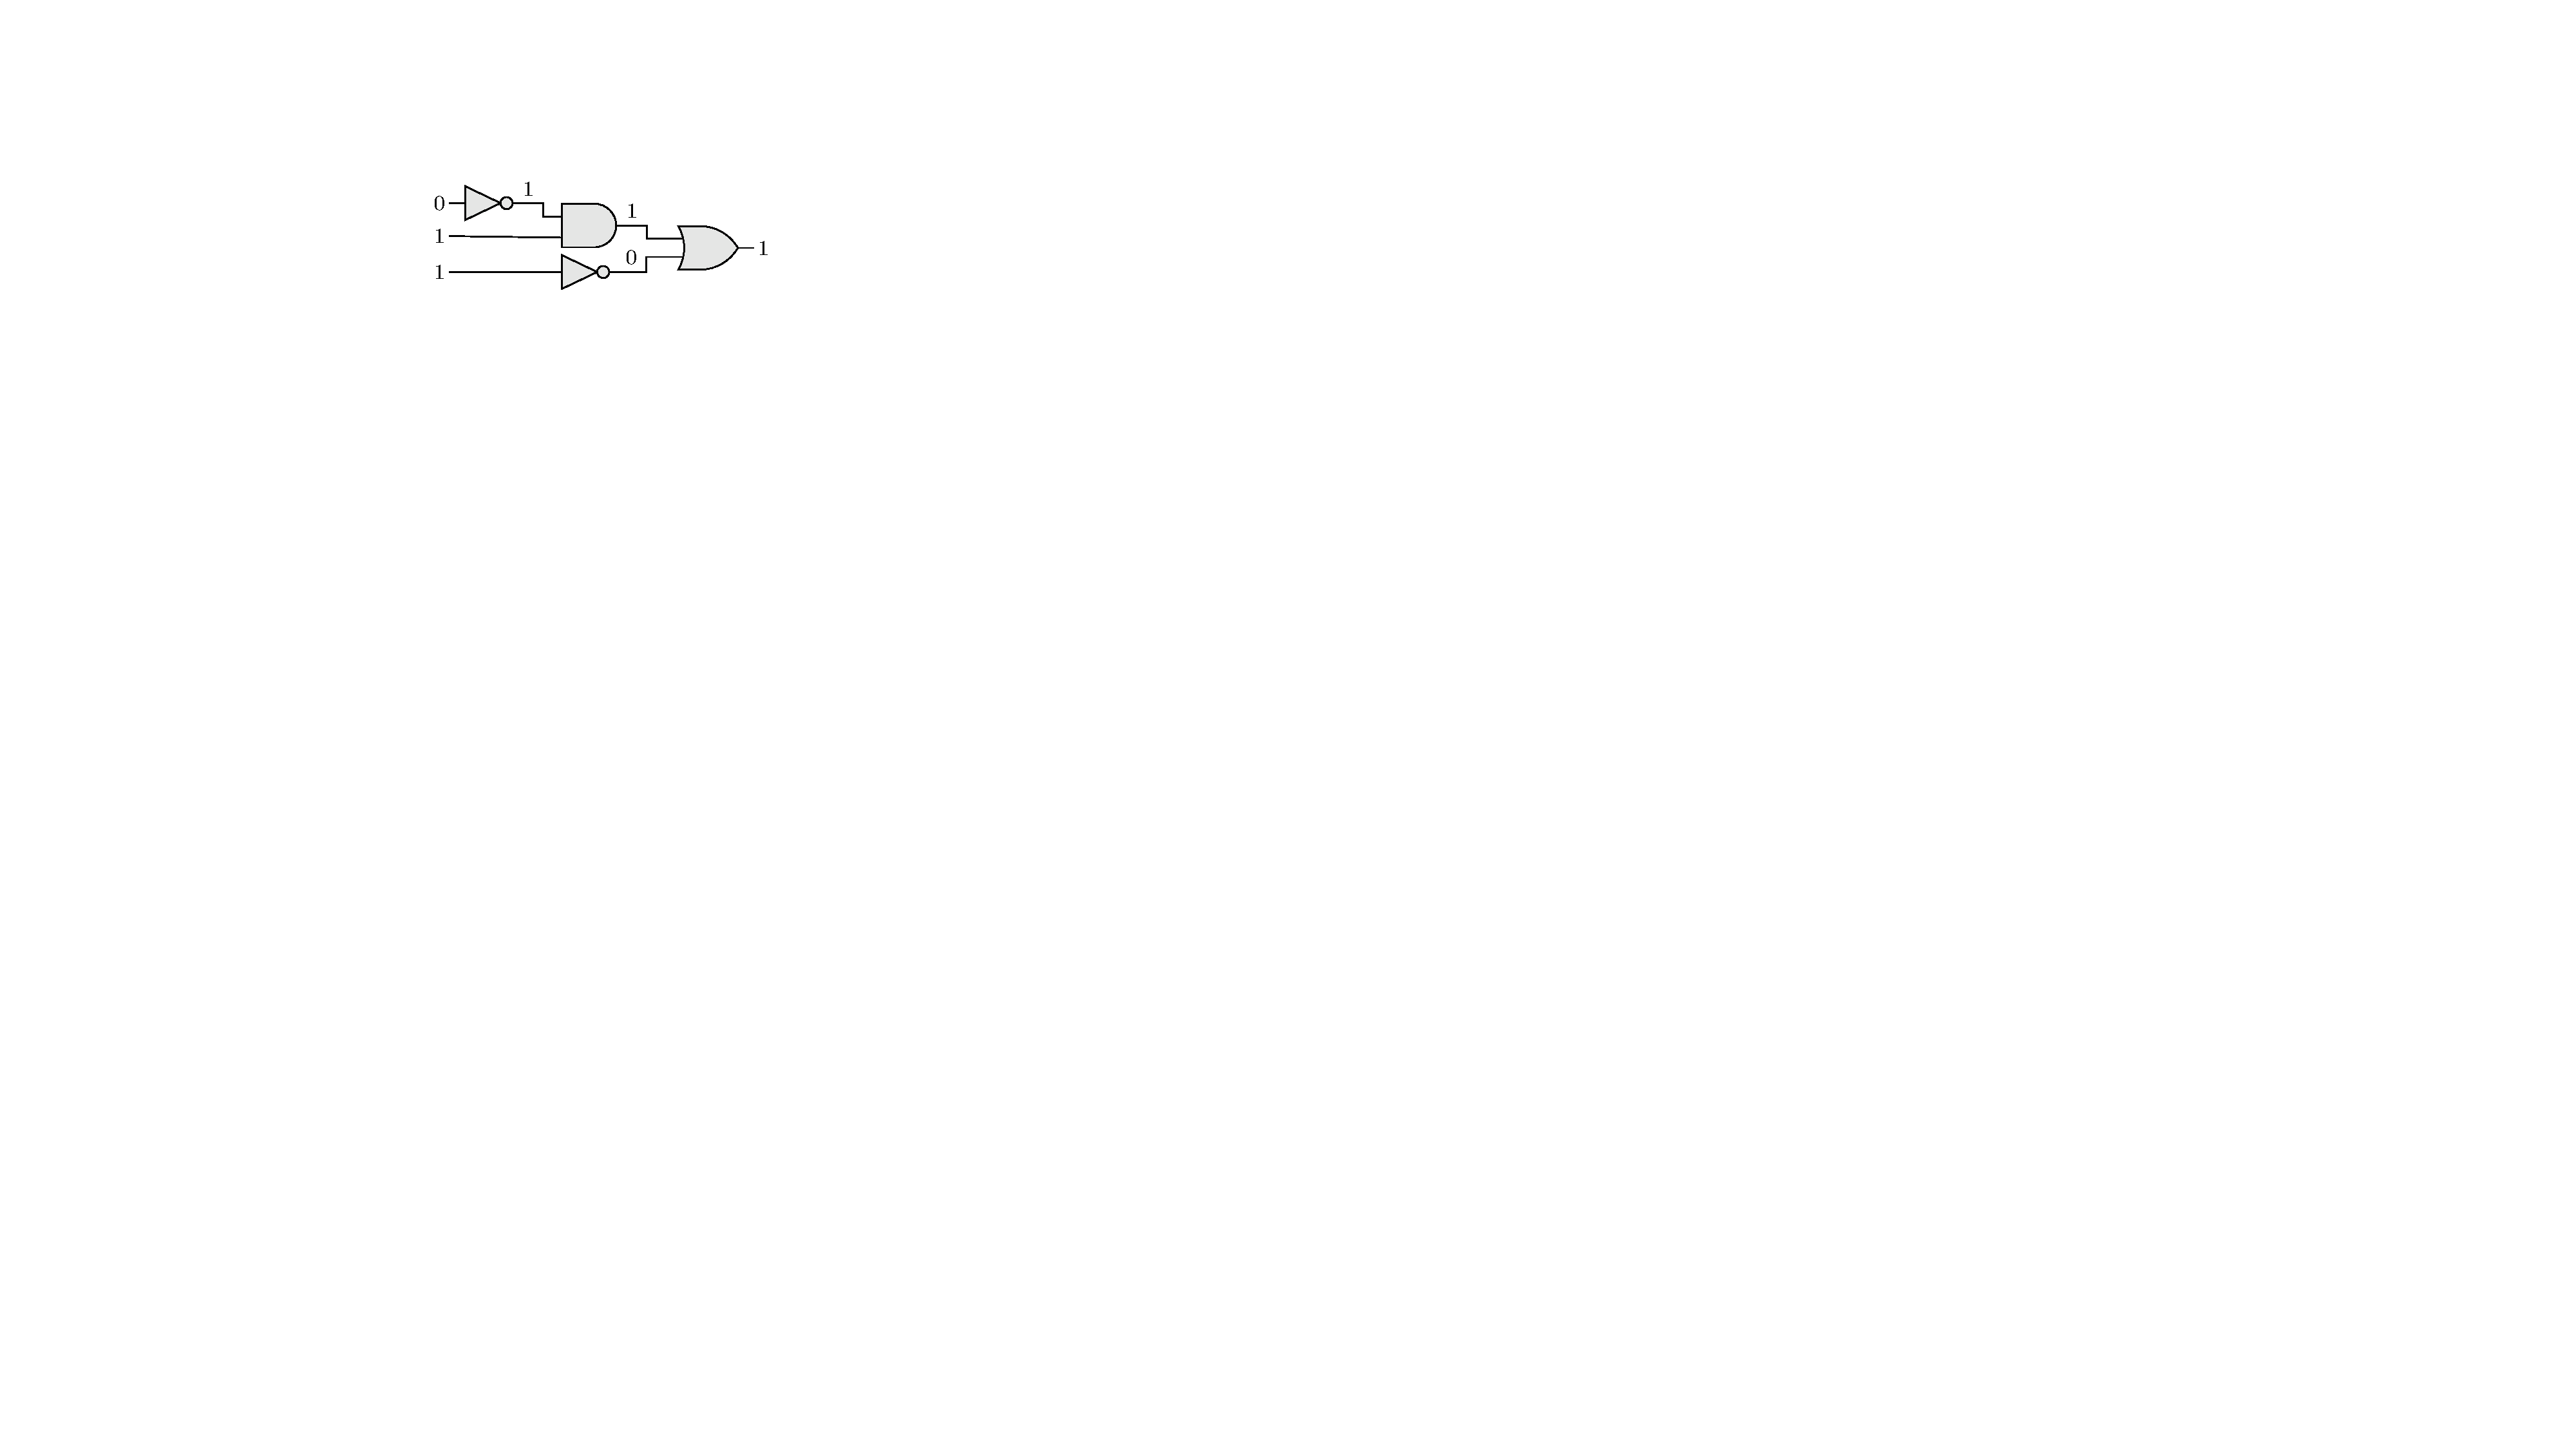
\includegraphics[]{Figures/HWCircuits/DigitalCircuit} \end{figure}
\newcommand\bstate{b}
\newcommand\qustate{q}

\paragraph{Bits and Qubits}
In classical computing, bits are the basic units of information. 
%
They can only be in one of two states: 0 or 1. 
%
We can think of them as switches that are either on or off. 
%
In contrast, quantum computing uses quantum bits, called {\it qubits}, to store information. Qubits can be in a state of 0, 1, or both simultaneously, a phenomenon known as {\it superposition}. 
%
Superposition allows quantum circuits to encode information more efficiently than classical circuits. 
%
Furthermore, qubits can be {\it entangled}: the state of one qubit is connected to another. 
%
Entaglement means the state of one qubit can't be described independently of the others.

\paragraph{Gates}
Logical gates, such as AND, OR, and NOT, are the fundamental components of digital circuits. 
%
They take binary inputs (0s and 1s) and produce a single binary output.
%
Each type of gate implements a specific binary function, e.g., the output of an AND gate is the conjunction of its inputs.
%
Quantum gates like the Hadamard and CNOT are the building blocks of quantum circuits, similar to classical logic gates. They manipulate qubits through unitary operations, allowing for quantum algorithms. Each gate performs a specific transformation, enabling superposition, entanglement, and measurement, thus enabling more complex computations compared to classical gates.

\paragraph{States}
The state of a sequence of bits is often represented by listing their values. For example, the input state in the figure is 011, indicating the values of the three input bits. Generally, $n$ bits can have $2^n$ possible states. 
%

In quantum computing, bits and states have a richer structure.
%
A {\it basis state} for a quantum bit is one of the classical states $0$ or $1$.
%
A qubit can be in a basis state or, more generally, in a {\it superposition} of the basis states, represented mathematically as: $[|\psi⟩ = \alpha |0⟩ + \beta |1⟩ ]$.
Here, $\alpha$ and $\beta$ are complex coefficients that determine the probability of measuring the qubit in either state.
The probabilities are given by:
Probability of measuring $|0⟩$: $( |\alpha|^2 )$
Probability of measuring $|1⟩$: $( |\beta|^2 )$
The condition $( |\alpha|^2 + |\beta|^2 = 1 )$ must hold to ensure valid probabilities.
%
In a system with $\nn$ qubits, there are $2^\nn$ possible basis states.
%
In general, a quantum state is a superposition of a set of basis state, representing a probability distribution over the possible $2^n$ bit-assignments.
%
A quantum state $\qustate$ assignes to each basis state $\bstate$ a complex number $\alpha_\bstate$ called the {\it amplitude} of $\bstate$ in $\qustate$.
%
Intuitively, if we \patodo{measure} $\qustate$ then the probability that we observe $\bstate$ is given by the square $\alpha_\bstate^2$ iof thbe amplitude.
%
The a
The left side of \cref{qustate:tree:fig} shows a quantum state with three qubits.
%
Each row of the table gives the amplitude of one basis state.
%


\paragraph{Circuits}
A combinatorial circuit consists of a set of gates and acts as a Boolean function. It takes a sequence of bits as input and produces a sequence of bits as output. There are also internal bits that represent the connections between gates. In the figure, the circuit has three input bits, one output bit, and three internal bits.
\patodo{Describe quantum states}


The basis states represent the simplest forms of qubit states:
|0⟩: Represents the state where the qubit is definitively in the "0" position.
|1⟩: Represents the state where the qubit is definitively in the "1" position.
These states are often referred to as computational basis states.
3. Superposition

